\PassOptionsToPackage{unicode=true}{hyperref} % options for packages loaded elsewhere
\PassOptionsToPackage{hyphens}{url}
%
\documentclass[]{article}
\usepackage{lmodern}
\usepackage{amssymb,amsmath}
\usepackage{ifxetex,ifluatex}
\usepackage{fixltx2e} % provides \textsubscript
\ifnum 0\ifxetex 1\fi\ifluatex 1\fi=0 % if pdftex
  \usepackage[T1]{fontenc}
  \usepackage[utf8]{inputenc}
  \usepackage{textcomp} % provides euro and other symbols
\else % if luatex or xelatex
  \usepackage{unicode-math}
  \defaultfontfeatures{Ligatures=TeX,Scale=MatchLowercase}
\fi
% use upquote if available, for straight quotes in verbatim environments
\IfFileExists{upquote.sty}{\usepackage{upquote}}{}
% use microtype if available
\IfFileExists{microtype.sty}{%
\usepackage[]{microtype}
\UseMicrotypeSet[protrusion]{basicmath} % disable protrusion for tt fonts
}{}
\IfFileExists{parskip.sty}{%
\usepackage{parskip}
}{% else
\setlength{\parindent}{0pt}
\setlength{\parskip}{6pt plus 2pt minus 1pt}
}
\usepackage{hyperref}
\hypersetup{
            pdftitle={Draft project on CAP modeling},
            pdfauthor={François Deloche},
            pdfborder={0 0 0},
            breaklinks=true}
\urlstyle{same}  % don't use monospace font for urls
\usepackage[margin=1in]{geometry}
\usepackage{graphicx,grffile}
\makeatletter
\def\maxwidth{\ifdim\Gin@nat@width>\linewidth\linewidth\else\Gin@nat@width\fi}
\def\maxheight{\ifdim\Gin@nat@height>\textheight\textheight\else\Gin@nat@height\fi}
\makeatother
% Scale images if necessary, so that they will not overflow the page
% margins by default, and it is still possible to overwrite the defaults
% using explicit options in \includegraphics[width, height, ...]{}
\setkeys{Gin}{width=\maxwidth,height=\maxheight,keepaspectratio}
\setlength{\emergencystretch}{3em}  % prevent overfull lines
\providecommand{\tightlist}{%
  \setlength{\itemsep}{0pt}\setlength{\parskip}{0pt}}
\setcounter{secnumdepth}{5}
% Redefines (sub)paragraphs to behave more like sections
\ifx\paragraph\undefined\else
\let\oldparagraph\paragraph
\renewcommand{\paragraph}[1]{\oldparagraph{#1}\mbox{}}
\fi
\ifx\subparagraph\undefined\else
\let\oldsubparagraph\subparagraph
\renewcommand{\subparagraph}[1]{\oldsubparagraph{#1}\mbox{}}
\fi

% set default figure placement to htbp
\makeatletter
\def\fps@figure{htbp}
\makeatother

\usepackage[]{natbib}
\bibliographystyle{plainnat}

\title{Draft project on CAP modeling}
\author{François Deloche}
\date{March 19, 2020}

\begin{document}
\maketitle

\hypertarget{elements-from-previous-work}{%
\section{Elements from previous
work}\label{elements-from-previous-work}}

Note: Good review article on CAP\\
\emph{Ups and downs in 75 years of electrocochleography} Eggermont
\citep{Eggermont2017}.

\hypertarget{the-narrow-band-contributions-to-the-compound-action-potential}{%
\subsection{The narrow-band contributions to the compound action
potential}\label{the-narrow-band-contributions-to-the-compound-action-potential}}

Masking of a click or tone-burst with a high-passed white noise (NB: not
strictly speaking forward masking as the noise was kept during the
probe, as far as I understand). The subtraction of the CAP obtained with
masking with the previous recording (\(f_{cut}\) cut-off frequency
decreases at each step) gives the `narrow-band' contribution of the CAP.

It has been used especially by Eggermont, although not the 1st one to
use it (Teas et al., 1962)

\begin{itemize}
\tightlist
\item
  \emph{Analysis of compound action potential responses to tone bursts
  in the human and guinea pig cochlea} Eggermont 1976
  \citep{Eggermont1976}

  \begin{itemize}
  \tightlist
  \item
    TT recordings
  \end{itemize}
\item
  \emph{Narrow-band analysis of compound action potentials for several
  stimulus conditions in the guinea pig} Eggermont 1981
\end{itemize}

\begin{figure}
\centering
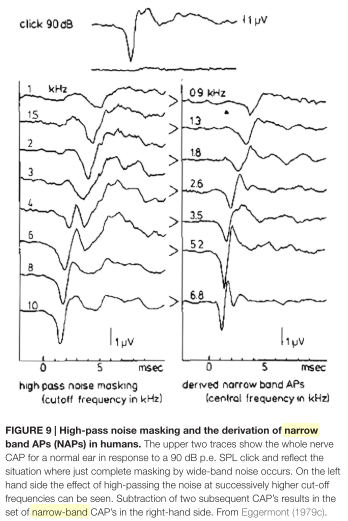
\includegraphics[width=4in,height=\textheight]{./figures/NAP_click.png}
\caption{NAP of click in humans}
\end{figure}

\begin{figure}
\centering
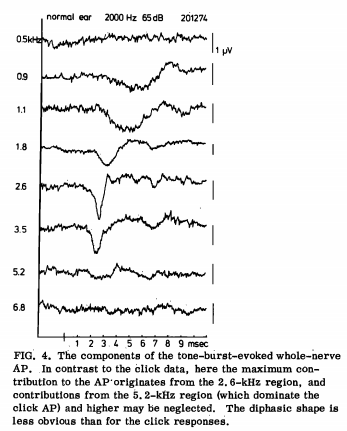
\includegraphics[width=3in,height=\textheight]{./figures/NAP_tone.png}
\caption{NAP of tone burst in humans. Eggermont 1976}
\end{figure}

\clearpage

Note: He found quite a different pattern for NAP in response to tone
bursts in guinea pigs (second negative peak)

\begin{figure}
\centering
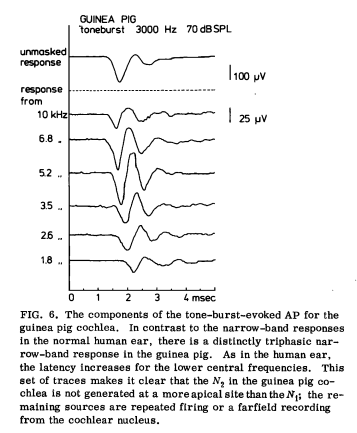
\includegraphics[width=3in,height=\textheight]{./figures/NAP_tone_guinea.png}
\caption{NAP of tone burst in guinea pigs. Eggermont 1976}
\end{figure}

Seems like we see a broader tuning of auditory filters.

\begin{itemize}
\tightlist
\item
  more frequencies contribute to the CAP
\item
  also the `narrow-band analysis' is less frequency selective. In fact,
  the `NAPs' do not show exactly the contribution of each frequency band
  because of the spread of the masker along the cochlear partition (this
  problem is alleviated in the model I propose because it seeks to
  estimate this spread with tuning of auditory filters)
\end{itemize}

\clearpage

The NAP method was used to estimate the latencies of each frequency
contribution:

\begin{figure}
\centering
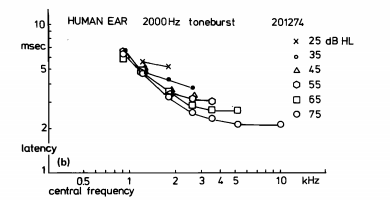
\includegraphics[width=4in,height=\textheight]{./figures/NAP_tone_latencies.png}
\caption{Latencies estimated with the NAP method}
\end{figure}

(exponential dependency on distance steps, more visible on this figure
for click : )

\begin{figure}
\centering
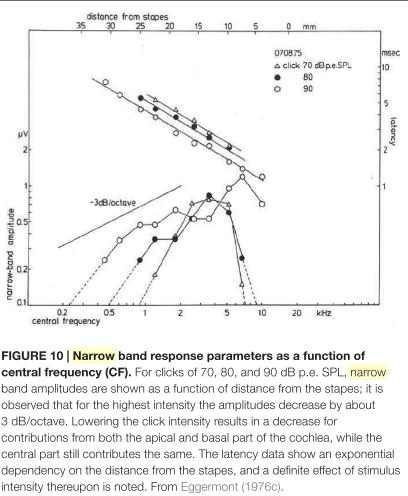
\includegraphics[width=4in,height=\textheight]{./figures/NAP_click_latencies.png}
\caption{Latencies estimated with the NAP method}
\end{figure}

\clearpage

\hypertarget{unit-responses-convolution-models}{%
\subsection{Unit responses, convolution
models}\label{unit-responses-convolution-models}}

\begin{itemize}
\tightlist
\item
  Individual ANF contribution
\end{itemize}

From Eggermont 2017 (review article):

\begin{quote}
Further experimental evidence for the applicability of the NAP technique
in pathological cochleas came from recordings in normal and
noise-exposed guinea pigs (Versnel et al., 1992), which looked at the
validity of using the same unit response along the CF range and in
normal vs.~hearing loss ears. They used a technique pioneered by Kiang
et al. (1976) involving spike-triggered averaging of round window
``noise''. In that way one can estimate the unit response for units with
CFs corresponding to locations along the cochlear partition. Their
findings in normal cochleas confirmed the earlier data from Prijs
(1986), namely that the unit response was diphasic and had a fairly
constant amplitude of about 0.1 µV. In noise-exposed cochleas, waveform,
latency and amplitude of the negative component of the unit response
remained unchanged.
\end{quote}

\begin{figure}
\centering
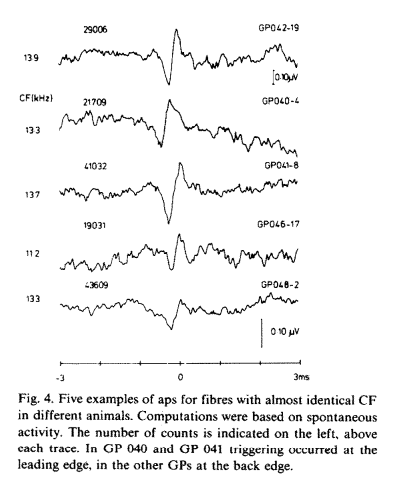
\includegraphics[width=3.5in,height=\textheight]{./figures/unit_response.png}
\caption{Unit response estimated with spike-triggered average, Prijs
1986 \citep{Prijs1986}}
\end{figure}

Similar to Kiang et al.~1976 \citep{Kiang1976}.

Other ref: thesis of Wang \citep{Wang1979}

\begin{figure}
\centering
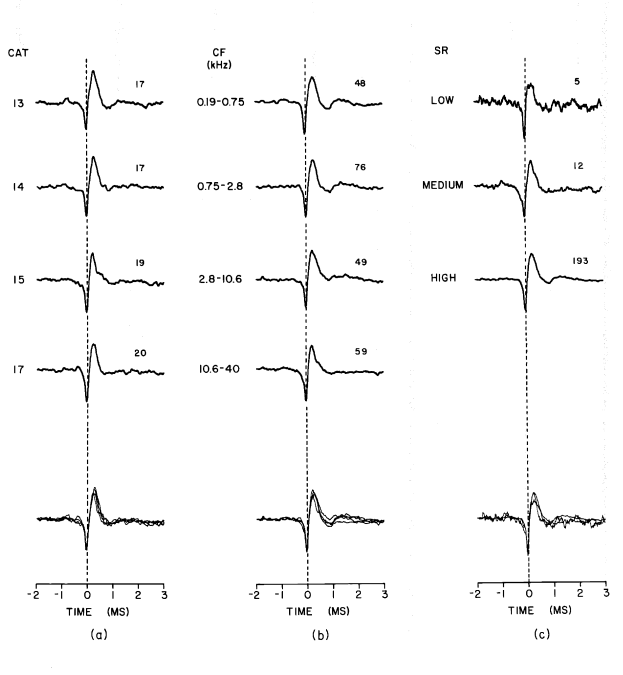
\includegraphics[width=5.5in,height=\textheight]{./figures/URs.png}
\caption{Fig 13 \citep{Wang1979} : averages of URs depending on animal,
CF, SR}
\end{figure}

\begin{figure}
\centering
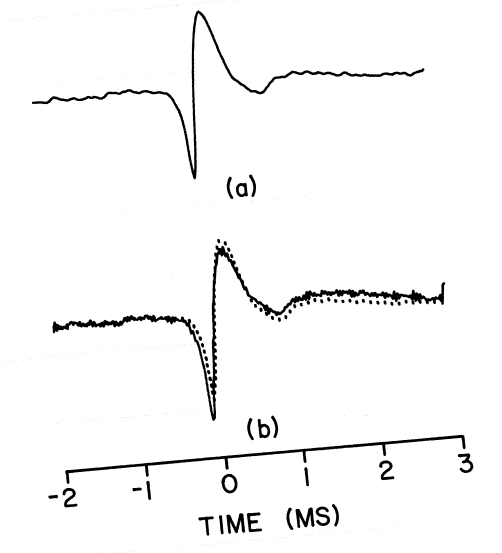
\includegraphics[width=2.5in,height=\textheight]{./figures/UR.png}
\caption{Fig 14 \citep{Wang1979} : full average}
\end{figure}

Note: interpretation in terms of finite differences:
\(\approx \delta - 2/1000 \delta'\) (and possibly second derivative)

\clearpage

\begin{itemize}
\tightlist
\item
  Synchronous fibers contribution
\end{itemize}

Related to the PST histogram or time distribution of first spike (if 2nd
peak negligible)

\begin{figure}
\centering
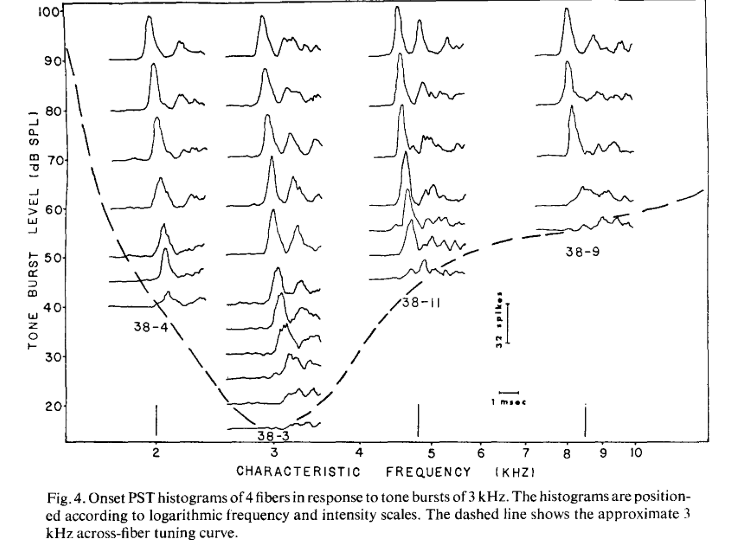
\includegraphics[width=5in,height=\textheight]{./figures/PST_tone.png}
\caption{Contributions of several ANFs at the onset of a tone.
\citep{Ozdamar1978}}
\end{figure}

\clearpage

\begin{itemize}
\item
  Double convolution models (or similar)

  \begin{itemize}
  \tightlist
  \item
    \emph{Synthetic whole-nerve action potentials for the cat} E. de
    Boer 1975 artifical PST histograms are computed with a filter +
    envelope + rectifier model, so it seems to go far in the modeling
  \item
    \emph{Deconvolution of compound action potentials and nonlinear
    features of the PST histogram} \citep{Bappert1980}
  \end{itemize}

  \[CAP = \underbrace{E \star NPST}_{CPST} \star UR\]

  CAP:Compound action potential\\
  E: excitation pattern (in time, does not try to go in the frequency
  domain using the latencies)\\
  NPST: ``norm'' PST (distribution of spikes for synchronous ANFs)\\
  CPST: Compound PST (PST given all the contributions of ANFs)\\
  UR: unit response\\
  In fact, there is a logarithm transform (dilatation) of the CPST to
  take into account the exponential shape of latencies wrt distance
  stapes, so it is not strictly speaking a double convolution.\\
  The model was used to estimate the excitation pattern.
\end{itemize}

\hypertarget{forward-masking-experiments}{%
\subsection{Forward masking
experiments}\label{forward-masking-experiments}}

\begin{itemize}
\tightlist
\item
  \emph{AP responses in forward-masking paradigms and relationship to
  responses of auditory-nerve fibers} Abbas, JASA 1981 \citep{Abbas1981}
\item
  Verschooten et al., 2012/2018 \citep{verschooten2012, Verschooten2018}
\item
  \emph{Forward masking of the compound action potential: Thresholds for
  the detection of the N1 peak} Relkin 1990 (deals with detection
  threshold and \% detection only) \citep{Relkin1991}
\end{itemize}

\begin{figure}
\centering
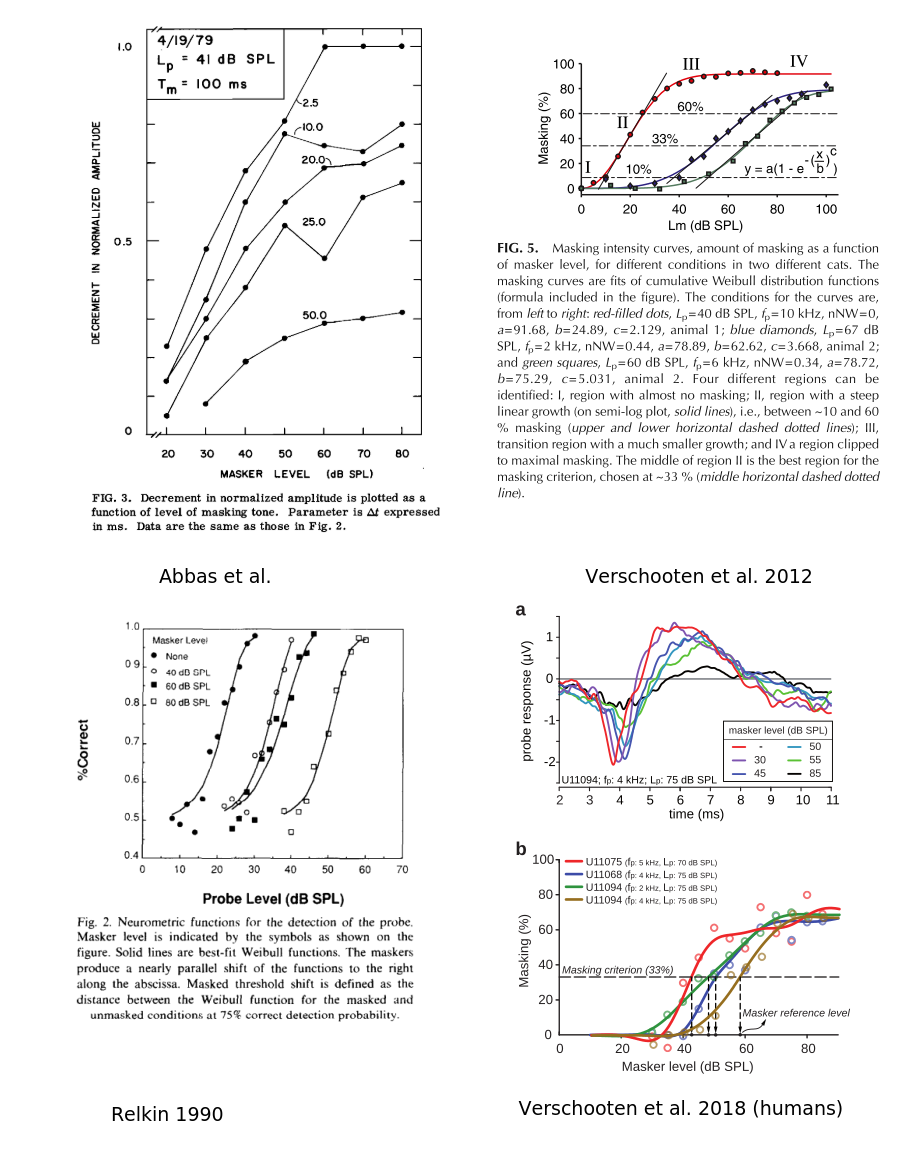
\includegraphics{./figures/forward_masking.png}
\caption{Forward masking: masking of CAP as a function of probe level
(in case of Verschooten et al.: broadband noise). Sometimes fit by a
Weibull function \label{fig:masking}}
\end{figure}

\begin{itemize}
\tightlist
\item
  estimation of tuning : Harrison 1981
  \citep{Harrison1981, Harrison1981a}, Verschooten et al.
\end{itemize}

\clearpage

\hypertarget{idea}{%
\section{Idea}\label{idea}}

\textbf{General idea: } return to the `double convolution' model but
exploit different forward masking settings to have a more robust model
of CAP (and possibly estimate auditory tuning)

\[CAP = \underbrace{E \star NPST}_{CPST} \star UR\]

(notations of \citep{Bappert1980}). Or:

\[CAP = E \star H\]

where \(E\) is the `excitation pattern' and \(H=NPST \star UR\). It's a
`blind deconvolution' problem because we have only a vague idea of what
\(E\) and \(H\) are.

With forward masking, we can get more information. Instead of having a
single excitation pattern \(E\), we can have several patterns

\[E_i = M_i (\theta) \cdot E_0\]

where \(M_i(\theta)\) is a masking pattern depending on the masker
(tone, band noise..), and \(E_0\) is the raw excitation pattern (without
masking). The masking pattern depends on the model parameters \(\theta\)
which are primarily the latencies and the frequency selectivity (given a
simple model of auditory filters). We can compute a theoretical `masking
pattern' thanks to the plot of \% masking as a function of masker level
for broadband noise, see Fig. \ref{fig:masking} (under certain
assumptions, e.g.~have to be careful of growth-of-masking).

Then now we have a system of equations with

\[[CAP]_i = [M_i (\theta) \cdot E_0]_i \star H \ .\]

It is still the `blind deconvolution' problem but we have a stronger
prior on the excitation patterns as they belong to a linear subspace
parametrized by \(E_0\). Simple projection-based algorithms exist in
this case \citep{Yang1994} (this is essentially deconvolution done
alternatively on \(E\) and \(H\) with a projection step between two
iterations). Note: prior constraints could be also put on \(H\) based on
what we know about UR and NPST, but this seems more challenging (maybe
as a second step). We can also think of a regularity prior on \(E_0\).\\
idea: initialize the algorithm with reasonable estimations of \(E\) and
\(H\). At the end of the algorithm, done for each set of parameters
\(\theta\), we would select the best model minimizing the square error,
then see how it behaves compared to real data.

Toy model: Masked CAP toy model.ipynb\\
Possibility of first step? try to see if estimation works on simple
simulated data like this one

\begin{itemize}
\tightlist
\item
  TODO, next week : more on type of makser/probes, hypotheses, questions
  and difficulties
\end{itemize}

\bibliography{biblioCAP.bib}

\end{document}
